\question Recall from the notes that a \textbf{rooted tree} is a tree 
with a particular node designated as the root, and the other nodes 
arranged in levels, “growing down” from the root. An alternative, 
recursive, definition of rooted tree is the following:  A rooted tree 
consists of a single node, the root, together with zero or more 
“branches,” each of which is itself a rooted tree. The root of the 
larger tree is connected to the root of each branch. \newline
\begin{figure}[h]
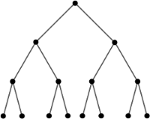
\includegraphics{rooted_tree}
\centering
\end{figure}\newline
Prove that given any tree, selecting any node to be the root produces 
a rooted tree according to the definition above.

\begin{solution}[1.5in]
Use induction! (on number of vertices)\newline
\textit{Base case}: one-vertex tree; have to select that to be the 
root; trivially a rooted tree (with zero branches)\newline
\textit{Inductive hypothesis}: tree with $k$ or fewer vertices can 
be made into rooted tree by selecting any vertex as root\newline
\textit{Inductive step}: given a tree with $k + 1$ vertices, let an 
arbitrary vertex $v$ be selected as the root. This vertex $v$ has, 
let us say, $m$ neighbors.\newline Disconnecting each neighbor from 
$k$ would produce $m$ subtrees (which must be disjoint, or else we 
would have a cycle). By the inductive hypothesis, because each of 
these has at most $k$ vertices, they each form a rooted tree when we 
select $v$’s neighbor as the root. Overall, then, we have a root node, 
$v$, connected to a number of disjoint rooted trees, which are its 
branches.
\end{solution}